% Slides for 2025-07-08
% To create a slide, use the following:
% \begin{frame}{TITLE}
%     BODY
% \end{frame}

\begin{frame}{ML Team Agenda}
    \begin{itemize}
        \item EGCI Work
        \item Literature Search for Public Data
        \item Vector Databases
        \item Binary Classifier
    \end{itemize}
\end{frame}

\begin{frame}{EGCI}
    
\end{frame}

\begin{frame}{Literature Search}
    \begin{itemize}
        \item Looking for more audio data for improved model performance
        \item Lin et al., 2021
        \begin{itemize}
            \item Healthy coral reef data off Sesoko Island, Okinawa, Japan
        \end{itemize}
        \item NOAA
        \begin{itemize}
            \item Various passive acoustic data from 30 marine recording sites
        \end{itemize}
        \item Williams et al., 2024
        \begin{itemize}
            \item Coral reef data from French Polynesia, Australia, \& Indonesia
        \end{itemize}
    \end{itemize}
    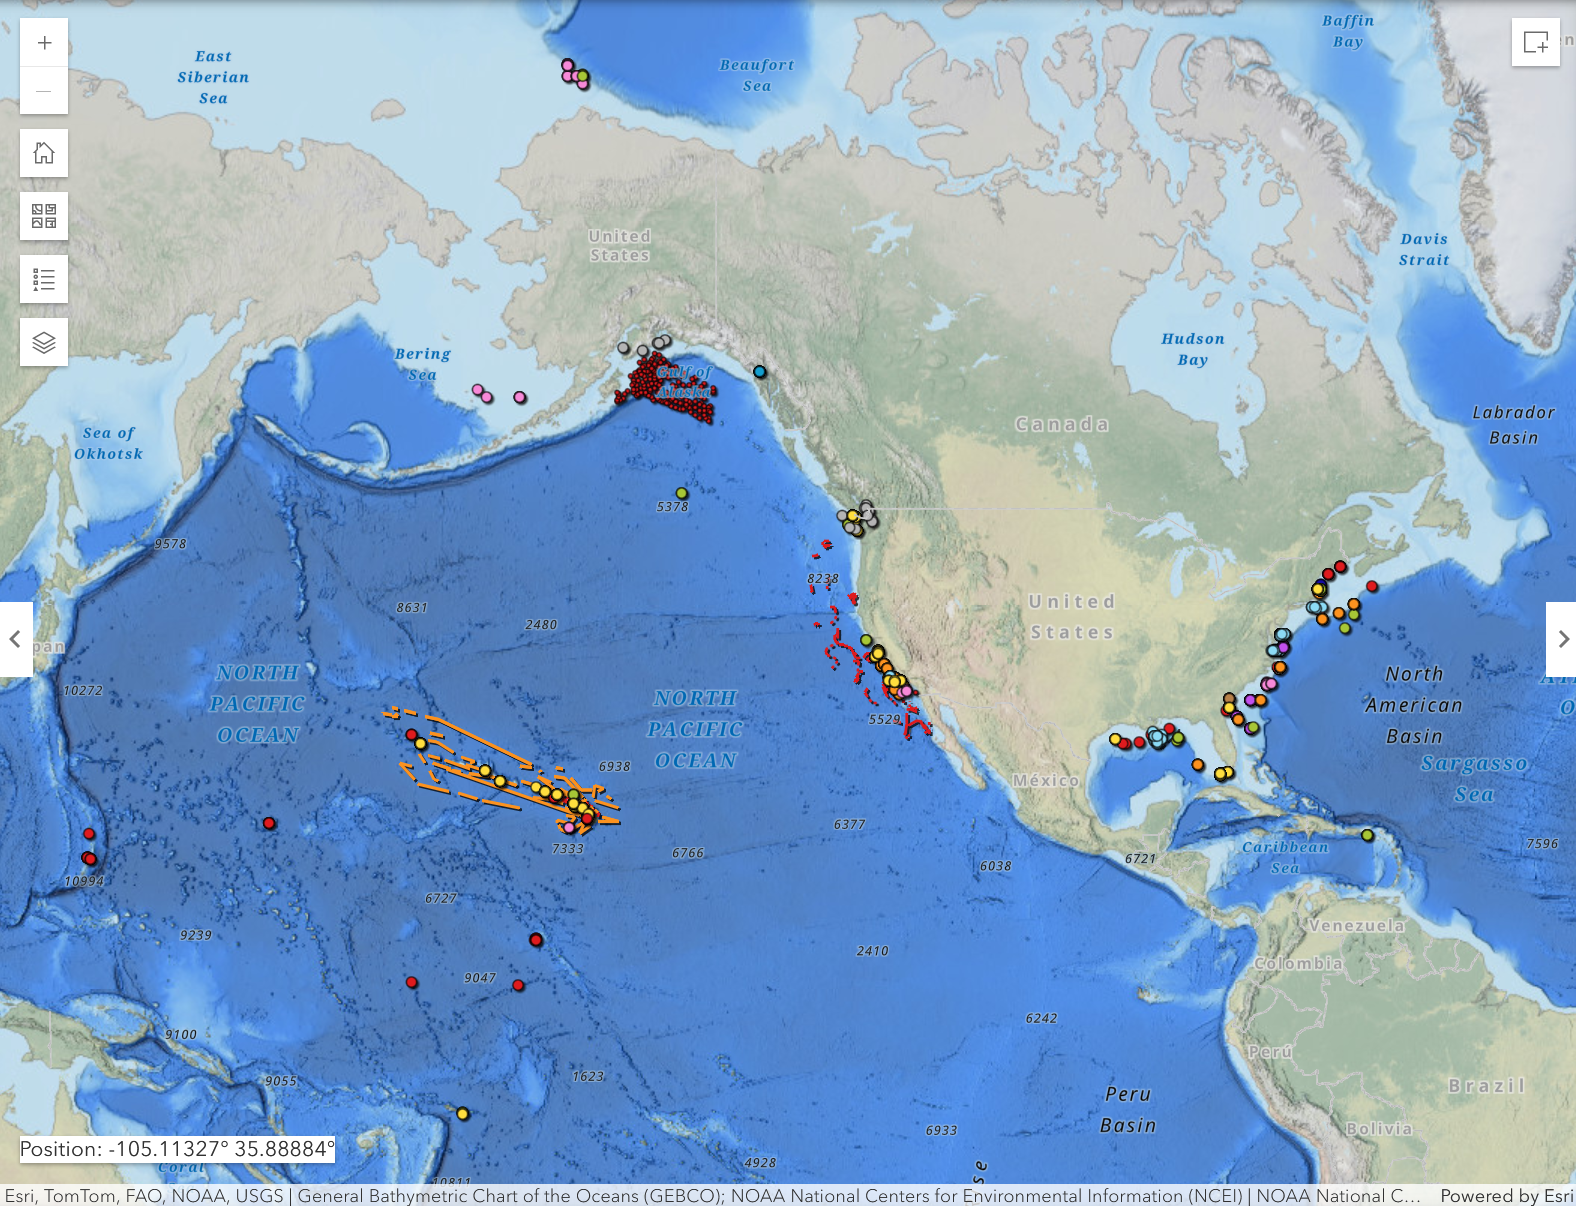
\includegraphics[height=0.4\textheight,width=0.7\textwidth,keepaspectratio]{images/aid_1.jpg}
    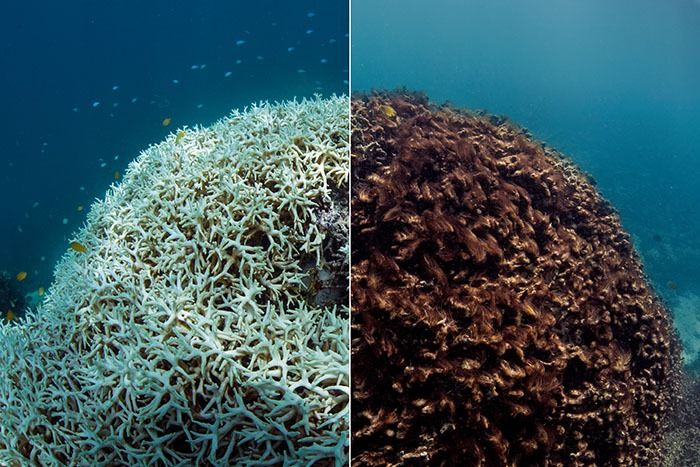
\includegraphics[height=0.4\textheight,width=0.7\textwidth,keepaspectratio]{images/aid_2.jpg}
\end{frame}

\begin{frame}{Vector Databases}
    \begin{itemize}
        \item Generated vector embeddings \& inserted into LanceDB, a vector database
        \item \textbf{Next Steps:} Explore TimeScale DB, a vector db with temporal and geospatial indexing
    \end{itemize}
    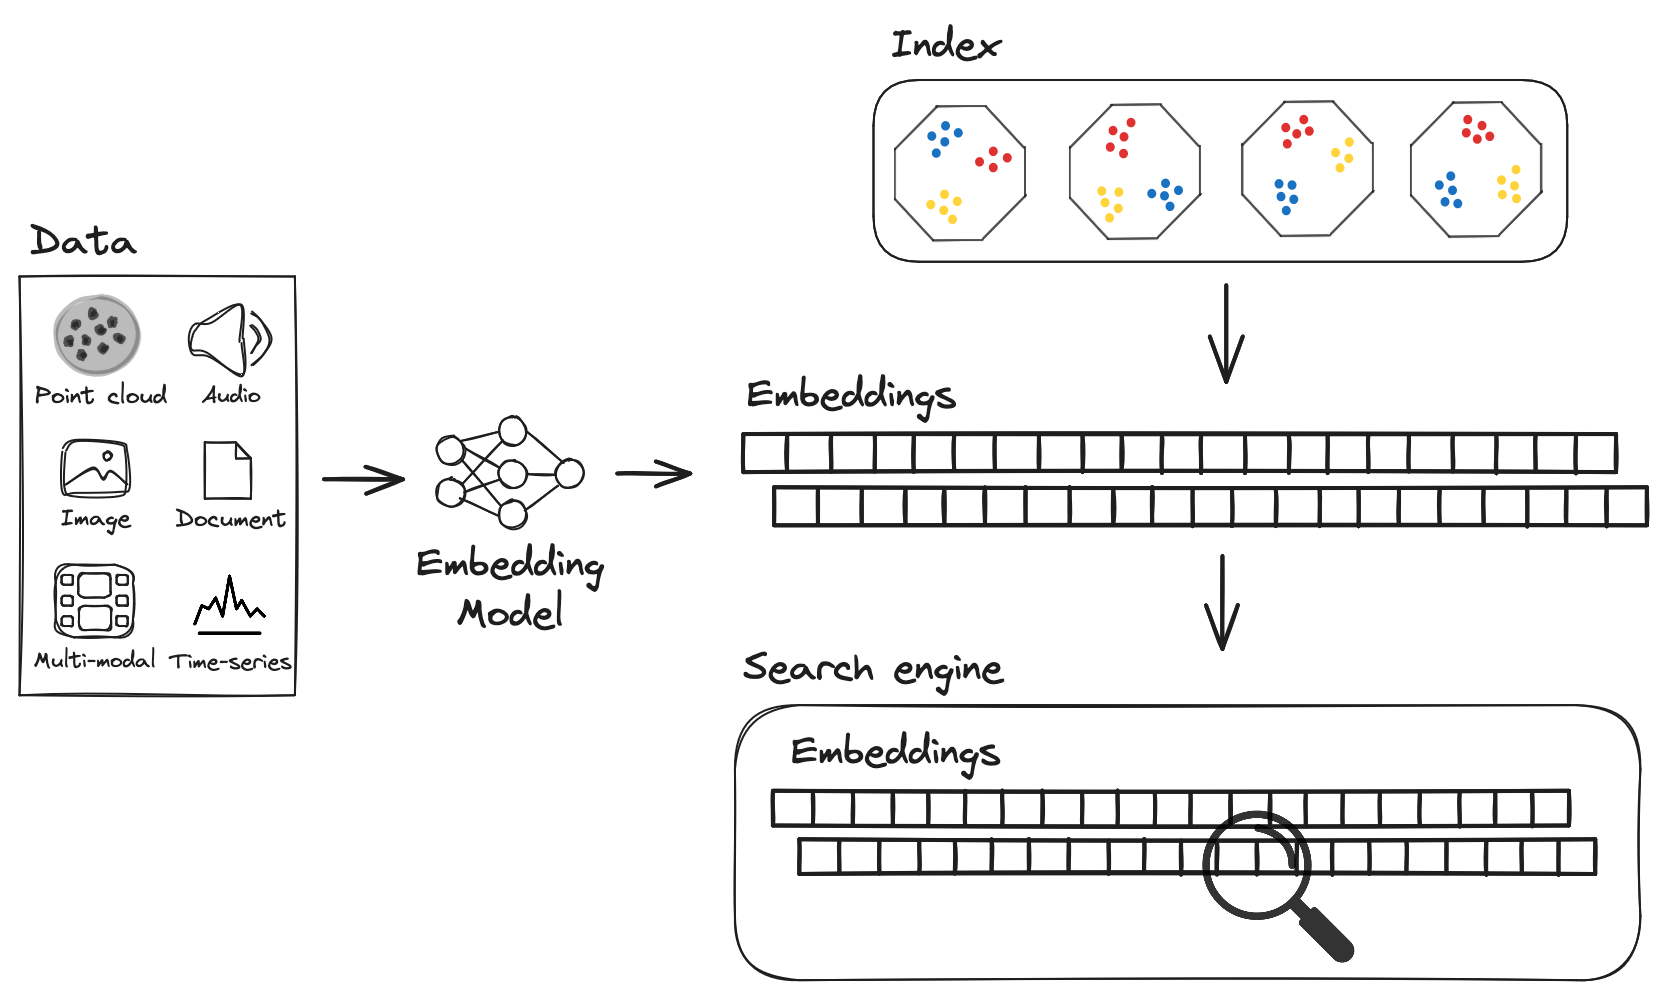
\includegraphics[height=0.4\textheight,width=0.7\textwidth,keepaspectratio]{images/aid_lancedb_1.png}
    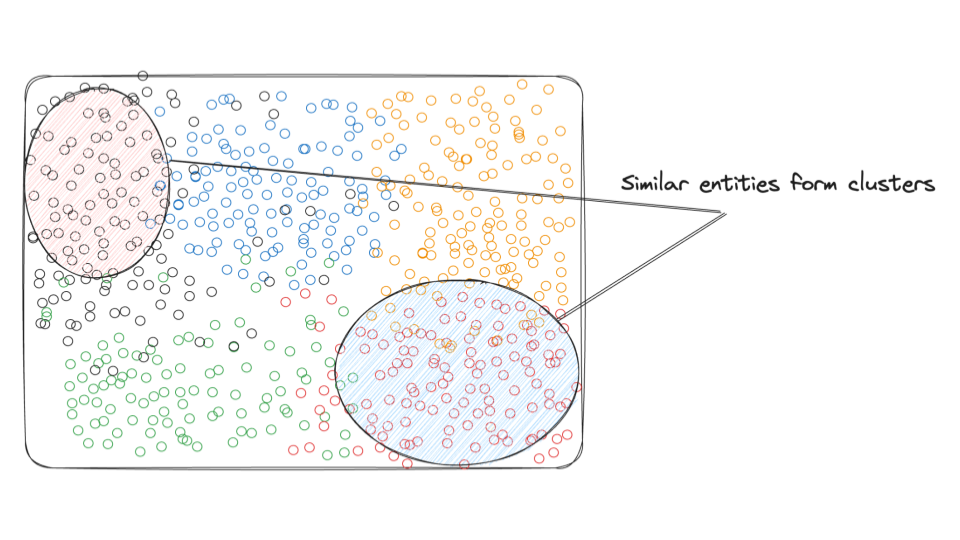
\includegraphics[height=0.4\textheight,width=0.7\textwidth,keepaspectratio]{images/aid_lancedb_2.png}
\end{frame}

\begin{frame}{Binary Classifier}
    \begin{itemize}
        \item Ran pre-existing multilabel classifier to determine degraded or non degraded reef
        \item Training Results:
    \end{itemize}
    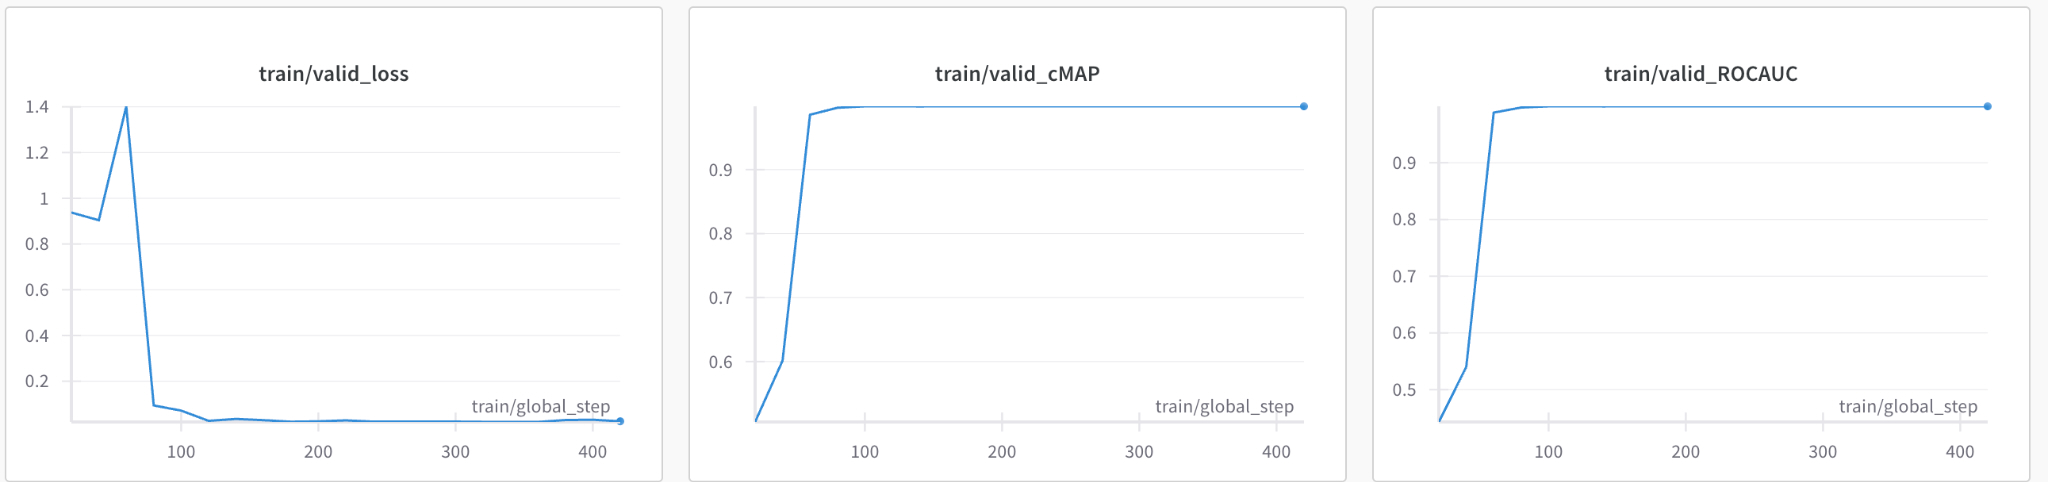
\includegraphics[height=0.4\textheight,width=0.7\textwidth,keepaspectratio]{images/aid_training_results.jpg}
    \begin{itemize}
        \item Testing Results: 
        \begin{itemize}
            \item cMAP: 0.99883
            \item ROCAUC: 0.999433
        \end{itemize}
        \item \textbf{Next Steps:} GradCAM, to visualize model predictions  
    \end{itemize}  
\end{frame}

\begin{frame}{Collar Team Agenda}
    \begin{itemize}
        \item Power Studies
        \begin{itemize}
            \item Power Study Overview
            \item Test Setup 
            \item In-rush Current Measurements
            \item Run Mode Configuration Measurements
        \end{itemize}
        \item Data Loss
        \begin{itemize}
            \item 
        \end{itemize}
        \item Future Plans
    \end{itemize}
\end{frame}
     
\begin{frame}{Power Study Overview}
    \begin{itemize}
        \item Understand power behaviour of STM32H747I-DISCO chip
        \item Measure various runtime domains for collar design metrics
        \item Combine measurements for a total power consumption estimation
    \end{itemize}
\end{frame}

\begin{frame}{Test Setup}
    \begin{itemize}
        \item Measurements taken using current clamp and pico oscilloscope
        \item Power configurations tested: Run, Sleep, Standby, Dstandby
        \item Drift issue encountered → added 10 Ohms shunt resistor in parallel with IDD
        \item Current calculated using Vdrop across resistor / 10 Ohms
    \end{itemize}  
    % add image of test setup
    % \includegraphics[height=0.4\textheight,width=0.7\textwidth,keepaspectratio]{images/.png}
    % add image of setup schematic
    % \includegraphics[height=0.4\textheight,width=0.7\textwidth,keepaspectratio]{images/.png}
\end{frame}

\begin{frame}{In-Rush Current Measurements}
\begin{columns}

    % Left column: image
    \begin{column}{0.6\textwidth}
        \centering
        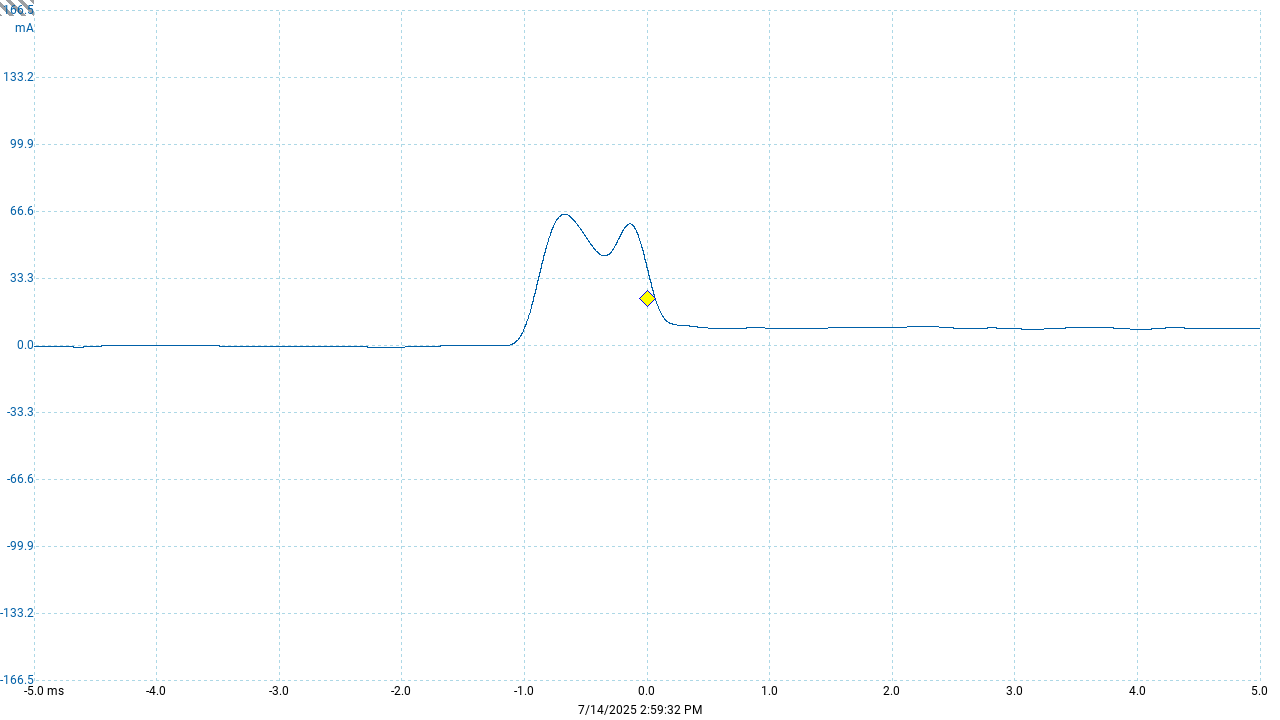
\includegraphics[width=\linewidth]{images/inrush_1core_baseline.png}
        \vspace{0.5em}
        {\small \textit{In-rush current spike at startup}}
    \end{column}

    % Right column: table
    \begin{column}{0.45\textwidth}
        \centering
        \begin{tabular}{|l|c|}
            \hline
            \textbf{Metric} & \textbf{Value} \\
            \hline
            Avg In-rush Peak 1 & 63.53 mA \\
            Avg In-rush Trough & 42.46 mA \\
            Avg In-rush Peak 2 & 58.27 mA \\
            Avg Duration     & 1.20 ms \\
            Method           & Current Clamp \\
            Trials           & 5 \\
            \hline
        \end{tabular}
        \vspace{0.5em}
        {\small \textit{In-rush Average Metrics}}
    \end{column}
\end{columns}
\end{frame}

\begin{frame}{Run Mode Configuration Measurements}
    \begin{itemize}
        \item 
    \end{itemize}
    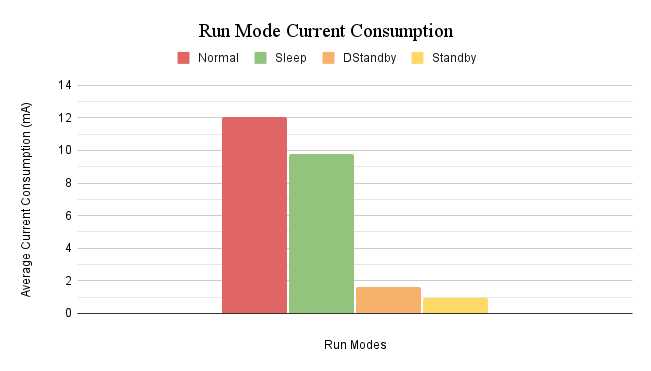
\includegraphics[height=0.5\textheight,width=0.9\textwidth,keepaspectratio]{images/run_modes.png}
\end{frame}
    
% To create a slide with a bullet list, use the following:
% \begin{frame}{TITLE}
%     \begin{itemize}
%         \item ITEM 1
%         \item ITEM 2
%     \end{itemize}    
% \end{frame}

% To create a slide with numbered list, use the following:
% \begin{frame}{TITLE}
%     \begin{enumerate}
%         \item ITEM 1
%         \item ITEM 2
%     \end{enumerate}
% \end{frame}

% To create a slide with a graphic:
% 1. Add the graphic to this folder (named picture.png)
% 2. Use the following:
% \begin{frame}{TITLE}
%     \centering
%     \includegraphics[height=0.7\textheight,width=0.7\textwidth,keepaspectratio]{picture.png}
% \end{frame}

% To create a slide with two columns, use the following:
% \begin{frame}{TITLE}
%     \begin{columns}
%         \begin{column}{0.5\textwidth}
%             COLUMN 1 BODY
%         \end{column}
%         \begin{column}{0.5\textwidth}
%             COLUMN 2 BODY
%         \end{column}
%     \end{columns}
% \end{frame}
